\begin{center}

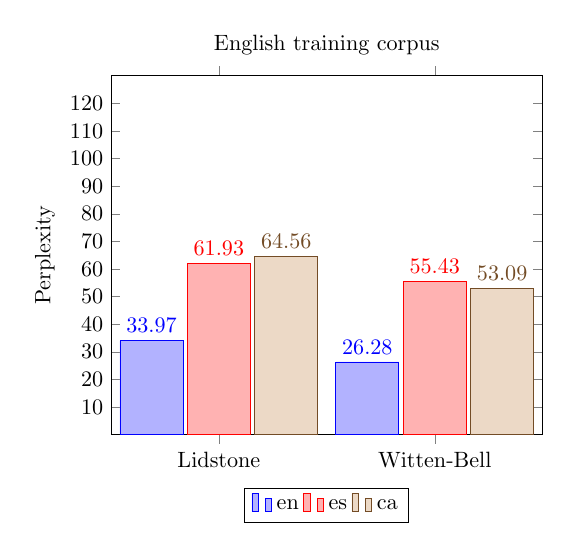
\begin{tikzpicture}[scale=.8]
\begin{axis}[
	title={English training corpus},
	ybar,
	enlarge x limits=0.5,
	legend style={at={(0.5,-0.15)}, anchor=north,legend columns=-1},
	ylabel={Perplexity},
	symbolic x coords={Lidstone,Witten-Bell},
	xtick=data,
	ymin=0, ymax=130,
	ytick={10,20,30,40,50,60,70,80,90,100,110,120},
	bar width=1cm,
	nodes near coords,
]
\addplot coordinates {(Lidstone,33.9709175258568834) (Witten-Bell,26.2813386380639109)};
\addplot coordinates {(Lidstone,61.9293643231486683) (Witten-Bell,55.4296898751559795)};
\addplot coordinates {(Lidstone,64.5575648340690549) (Witten-Bell,53.0874135920790380)};
\legend{en,es,ca}
\end{axis}
\end{tikzpicture}
\qquad
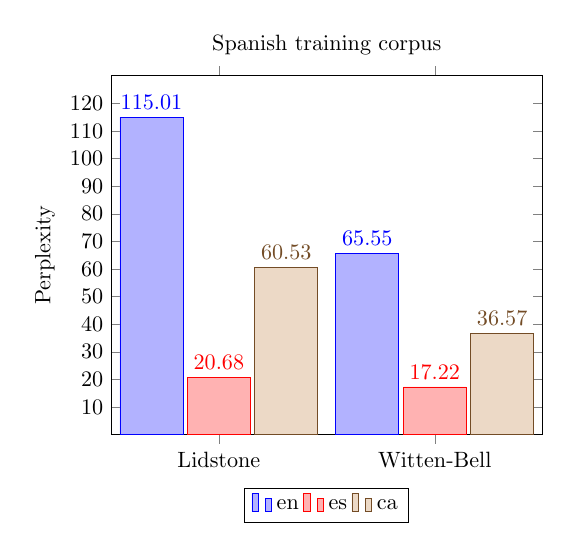
\begin{tikzpicture}[scale=.8]
\begin{axis}[
	title={Spanish training corpus},
	ybar,
	enlarge x limits=0.5,
	legend style={at={(0.5,-0.15)}, anchor=north,legend columns=-1},
	ylabel={Perplexity},
	symbolic x coords={Lidstone,Witten-Bell},
	xtick=data,
	ymin=0, ymax=130,
	ytick={10,20,30,40,50,60,70,80,90,100,110,120},
	bar width=1cm,
	nodes near coords,
]
\addplot coordinates {(Lidstone,115.0053619565369729) (Witten-Bell,65.5467578637442472)};
\addplot coordinates {(Lidstone,20.6760031479876538) (Witten-Bell,17.2177660276275013)};
\addplot coordinates {(Lidstone,60.5286457523718013) (Witten-Bell,36.5671173426087606)};
\legend{en,es,ca}
\end{axis}
\end{tikzpicture}

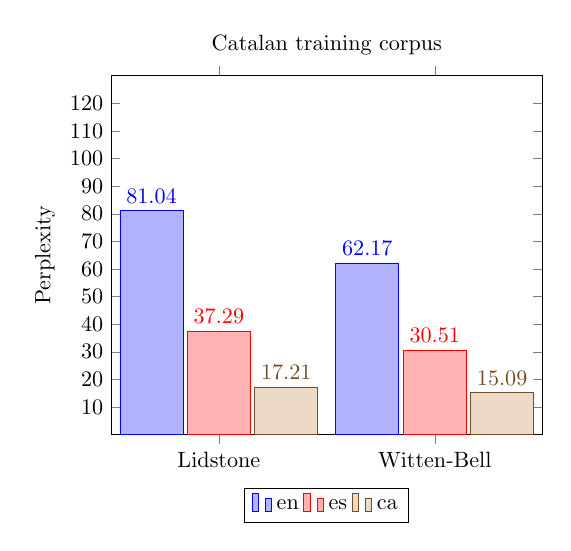
\begin{tikzpicture}[scale=.8]
\begin{axis}[
	title={Catalan training corpus},
	ybar,
	enlarge x limits=0.5,
	legend style={at={(0.5,-0.15)}, anchor=north,legend columns=-1},
	ylabel={Perplexity},
	symbolic x coords={Lidstone,Witten-Bell},
	xtick=data,
	ymin=0, ymax=130,
	ytick={10,20,30,40,50,60,70,80,90,100,110,120},
	bar width=1cm,
	nodes near coords,
]
\addplot coordinates {(Lidstone,81.0364047755355870) (Witten-Bell,62.1660478904621527)};
\addplot coordinates {(Lidstone,37.2923115076113945) (Witten-Bell,30.5072434974184787)};
\addplot coordinates {(Lidstone,17.2084235331928639) (Witten-Bell,15.0877099149183511)};
\legend{en,es,ca}
\end{axis}
\end{tikzpicture}

\end{center}